\documentclass[10pt]{beamer}

\usepackage{amsfonts}
\usepackage{subfiles}
\usepackage[T2A]{fontenc}
\usepackage[utf8]{inputenc}
\usepackage[russian]{babel}

\usepackage{amsmath, amsfonts, amssymb, amsthm, mathtools, mathrsfs}
\usepackage{wasysym, dsfont}
\usepackage{graphicx}
\usepackage{float}
\usepackage{wrapfig}
\usepackage{subcaption}
\usepackage{multirow}
\usepackage{caption}
\usepackage{subcaption}
\usepackage{xcolor}
% \usepackage{subfigure}

\usepackage{multicol}
\DeclareMathOperator*{\argmax}{\arg\!\max}
\DeclareMathOperator*{\argmin}{\arg\!\min}

\mode<presentation>
{
	\usetheme{boxes}
	\beamertemplatenavigationsymbolsempty{}
	
	\setbeamertemplate{footline}[page number]
	\setbeamersize{text margin left=1em, text margin right=1.5em}
}
\newcommand\blfootnote[1]{%
	\begingroup
	\renewcommand\thefootnote{}\footnote{#1}%
	\addtocounter{footnote}{-1}%
	\endgroup
}
\newcommand\FontUP{\fontsize{12}{12}\selectfont}


\title[]{Low rank attention denoising}

\author{Nikita Okhotnikov}

\institute{MIPT}
\date{2025}

\begin{document}

\begin{frame}
  \titlepage{}
\end{frame}


\begin{frame}
    \frametitle{Introduction}
    \begin{block}{Problem}
        \begin{itemize}
            \item Noisy attention weights distribution in modern LLMs hurts interpretability and potentially limits the performance
            \item Existing solution utilizes large number of additional parameters and requires training from scratch
        \end{itemize}
    \end{block}
    \begin{block}{Objective}
        Implement parameter and training time efficient attention score denoiser      
    \end{block}
    \begin{block}{Assumption}
        Attention noise has lower intrinsic dimensionality than the signal
    \end{block}
    \begin{block}{Proposal}
        Low rank implementation of existing adaptive denoiser\footnote{Yueyang Cang et al. DINT Transformer, 2025} that does not require training from scratch
    \end{block}
\end{frame}

\begin{frame}
    \frametitle{Attention \& DIFF attention}

    \begin{block}{Attention mechanism}
        \vspace{-0.5cm}

        $$X \in \mathbb{R}^{N \times d_{model}}\text{ -- input}, W_Q, W_K, W_V \in \mathbb{R}^{d_{model} \times d} \text{-- projection matrices}$$
        $$Q = X W_Q, K = X W_K, V = X W_V$$
        $$Q, K, V \in \mathbb{R}^{N \times d} \text{ -- projected queries, keys, values}$$
        $$\text{Attention} = \text{softmax}\left(\frac{Q K^T}{\sqrt{d}}\right) V$$

    \end{block}

    \begin{block}{DIFF attention mechanism}
        \vspace{-0.5cm}

        $$X \in \mathbb{R}^{N \times d_{model}}\text{ -- input}, W_Q, W_K \in \mathbb{R}^{d_{model} \times \textcolor{red}{2d}}, W_V \in \mathbb{R}^{d_{model} \times d}  \text{-- projection matrices}$$
        $$\textcolor{red}{[Q_1, Q_2] = X W_Q, [K_1, K_2] = X W_K}, V = X W_V$$
        $$Q_1, K_1, \textcolor{red}{Q_2, K_2}, V \in \mathbb{R}^{N \times d} \text{ -- projected queries, keys, values}$$
        $$\text{DIFFAttention} = \left(\text{softmax}\left(\frac{Q_1 K_1^T}{\sqrt{d}}\right) - \textcolor{red}{\lambda\cdot \text{softmax}\left(\frac{Q_2 K_2^T}{\sqrt{d}}\right)}\right)V, ~ \textcolor{red}{\lambda \in (0,1)}$$

    \end{block}

\end{frame}


\begin{frame}
    \frametitle{DINT Attention \& low rank modification}

    \begin{block}{DINT Attention}
        \vspace{-0.5cm}
        
        $$A_1 = \text{softmax}\left(\frac{Q_1 K_1^T}{\sqrt{d}}\right), A_2 = \text{softmax}\left(\frac{Q_2 K_2^T}{\sqrt{d}}\right), \textcolor{red}{A_3 = \text{repeat}\left(\frac{1}{N}\sum\limits_{i=1}^{N}A_1[i,:], N\right)}$$
        $$\text{DINTAttention} = \left(\textcolor{red}{\lambda\cdot A_3} + A_1 - \lambda\cdot A_2 \right) V$$

    \end{block}

    \begin{block}{Low rank DINT}
        \vspace{-0.5cm}

        $$Q_1 = X W_{Q_1}, K_1 = X W_{K_1}, \textcolor{red}{Q_2 = XW_{Q_2}^{down} W_{Q_2}^{up}, K_2 = XW_{K_2}^{down} W_{K_2}^{up}}$$
        $$W_{Q_1}, W_{K_1} \in \mathbb{R}^{d_{model} \times d}; \textcolor{red}{W_{Q_2}^{down}, W_{K_2}^{down} \in \mathbb{R}^{d_{model} \times r}; W_{Q_2}^{up}, W_{K_2}^{up} \in \mathbb{R}^{r \times d}} $$
        $$A_1 = \text{softmax}\left(\frac{Q_1 K_1^T}{\sqrt{d}}\right), A_2 = \text{softmax}\left(\frac{Q_2 K_2^T}{\textcolor{red}{\sqrt{d_2}}}\right), A_3 = \text{repeat}\left(\frac{1}{N}\sum\limits_{i=1}^{N}A_1[i,:], N\right)$$
        $$\text{ as linear layer of shape} [d_{in}, d_{out}] \text{ is initialized with } w[i,j] \sim U[-\sqrt{d_{in}}, \sqrt{d_{in}}]$$ $$\mathbb{D}[W_{Q_2}^{down} W_{Q_2}^{up}[i,j]] = \mathbb{D}[W_{K_2}^{down} W_{K_2}^{up}[i,j]] = \frac{1}{3 d_{model}}\cdot \frac{1}{3 r}\cdot r = \frac{1}{9}\mathbb{D}[W_{Q_1}[i,j]]$$
        $$\Longrightarrow \textcolor{red}{d_2 = \frac{d}{81}},~~ \text{LowRankDINTAttention} = \left(\lambda\cdot A_3 + A_1 - \lambda\cdot A_2 \right) V$$

    \end{block}
        
\end{frame}


\begin{frame}
    \frametitle{Preliminary experiments}

    SFT of Llama-3.2-1B model\footnote{https://huggingface.co/meta-llama/Llama-3.2-1B} on OpenMathInstruct-2 dataset\footnote{https://huggingface.co/datasets/nvidia/OpenMathInstruct-2}
    \begin{center}
        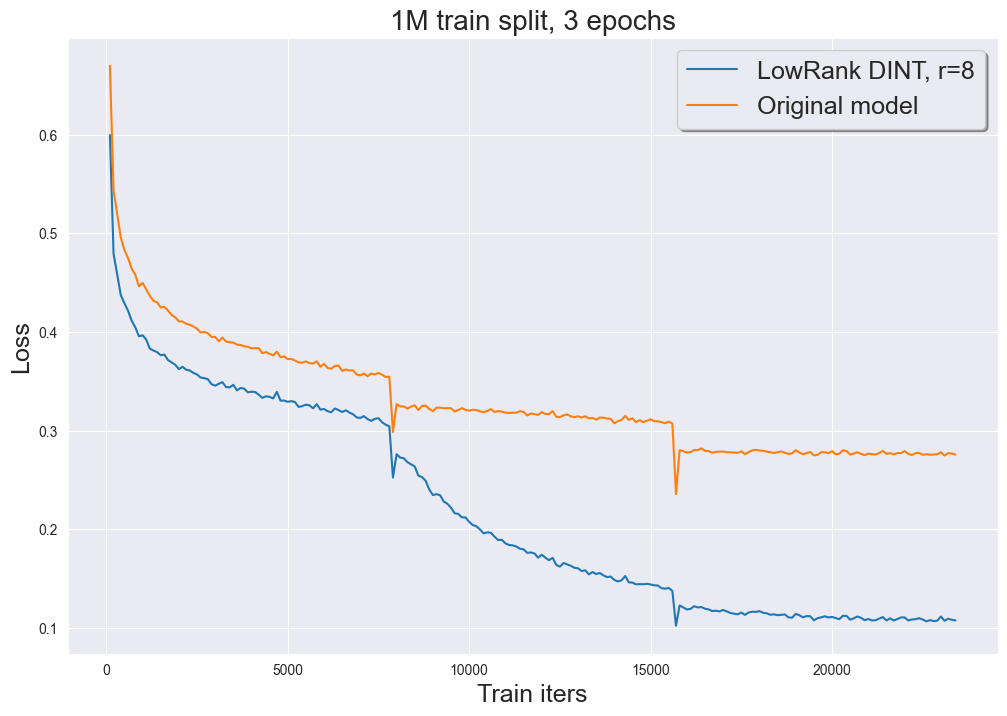
\includegraphics[scale=0.35]{../images/Loss_1M_3epochs.png}
    \end{center}
        
\end{frame}

\begin{frame}
    \frametitle{Preliminary results \& plans}
    \begin{block}{Observations}
        \begin{enumerate}
            \item Training loss value seems promising
            \item Test metrics are very questionable at the moment, might be a bug in the code
        \end{enumerate}
    \end{block}
    \begin{block}{Plans}
        \begin{enumerate}
            \item Examine testing pipeline
            \item Measure the entropy of attention weight distiribution, compare with original model
            \item Evaluate cross-domain impact of proposed denoiser
            \item Apply to larger models and different datasets
        \end{enumerate}
    \end{block}
\end{frame}


\end{document}
